% Options for packages loaded elsewhere
\PassOptionsToPackage{unicode,linktoc=all}{hyperref}
\PassOptionsToPackage{hyphens}{url}
\PassOptionsToPackage{dvipsnames,svgnames,x11names}{xcolor}
%
\documentclass[
  a4paper,
]{article}
\usepackage{amsmath,amssymb}
\usepackage{lmodern}
\usepackage{iftex}
\ifPDFTeX
  \usepackage[T1]{fontenc}
  \usepackage[utf8]{inputenc}
  \usepackage{textcomp} % provide euro and other symbols
\else % if luatex or xetex
  \usepackage{unicode-math}
  \defaultfontfeatures{Scale=MatchLowercase}
  \defaultfontfeatures[\rmfamily]{Ligatures=TeX,Scale=1}
\fi
% Use upquote if available, for straight quotes in verbatim environments
\IfFileExists{upquote.sty}{\usepackage{upquote}}{}
\IfFileExists{microtype.sty}{% use microtype if available
  \usepackage[]{microtype}
  \UseMicrotypeSet[protrusion]{basicmath} % disable protrusion for tt fonts
}{}
\makeatletter
\@ifundefined{KOMAClassName}{% if non-KOMA class
  \IfFileExists{parskip.sty}{%
    \usepackage{parskip}
  }{% else
    \setlength{\parindent}{0pt}
    \setlength{\parskip}{6pt plus 2pt minus 1pt}}
}{% if KOMA class
  \KOMAoptions{parskip=half}}
\makeatother
\usepackage{xcolor}
\IfFileExists{xurl.sty}{\usepackage{xurl}}{} % add URL line breaks if available
\IfFileExists{bookmark.sty}{\usepackage{bookmark}}{\usepackage{hyperref}}
\hypersetup{
  pdftitle={The Making of a Logo},
  pdfauthor={R (Chandra) Chandrasekhar},
  pdflang={en-GB},
  colorlinks=true,
  linkcolor={DarkOliveGreen},
  filecolor={Purple},
  citecolor={DarkKhaki},
  urlcolor={Maroon},
  pdfcreator={LaTeX via pandoc}}
\urlstyle{same} % disable monospaced font for URLs
\usepackage[margin=25mm]{geometry}
\usepackage{color}
\usepackage{fancyvrb}
\newcommand{\VerbBar}{|}
\newcommand{\VERB}{\Verb[commandchars=\\\{\}]}
\DefineVerbatimEnvironment{Highlighting}{Verbatim}{commandchars=\\\{\}}
% Add ',fontsize=\small' for more characters per line
\usepackage{framed}
\definecolor{shadecolor}{RGB}{48,48,48}
\newenvironment{Shaded}{\begin{snugshade}}{\end{snugshade}}
\newcommand{\AlertTok}[1]{\textcolor[rgb]{1.00,0.81,0.69}{#1}}
\newcommand{\AnnotationTok}[1]{\textcolor[rgb]{0.50,0.62,0.50}{\textbf{#1}}}
\newcommand{\AttributeTok}[1]{\textcolor[rgb]{0.80,0.80,0.80}{#1}}
\newcommand{\BaseNTok}[1]{\textcolor[rgb]{0.86,0.64,0.64}{#1}}
\newcommand{\BuiltInTok}[1]{\textcolor[rgb]{0.80,0.80,0.80}{#1}}
\newcommand{\CharTok}[1]{\textcolor[rgb]{0.86,0.64,0.64}{#1}}
\newcommand{\CommentTok}[1]{\textcolor[rgb]{0.50,0.62,0.50}{#1}}
\newcommand{\CommentVarTok}[1]{\textcolor[rgb]{0.50,0.62,0.50}{\textbf{#1}}}
\newcommand{\ConstantTok}[1]{\textcolor[rgb]{0.86,0.64,0.64}{\textbf{#1}}}
\newcommand{\ControlFlowTok}[1]{\textcolor[rgb]{0.94,0.87,0.69}{#1}}
\newcommand{\DataTypeTok}[1]{\textcolor[rgb]{0.87,0.87,0.75}{#1}}
\newcommand{\DecValTok}[1]{\textcolor[rgb]{0.86,0.86,0.80}{#1}}
\newcommand{\DocumentationTok}[1]{\textcolor[rgb]{0.50,0.62,0.50}{#1}}
\newcommand{\ErrorTok}[1]{\textcolor[rgb]{0.76,0.75,0.62}{#1}}
\newcommand{\ExtensionTok}[1]{\textcolor[rgb]{0.80,0.80,0.80}{#1}}
\newcommand{\FloatTok}[1]{\textcolor[rgb]{0.75,0.75,0.82}{#1}}
\newcommand{\FunctionTok}[1]{\textcolor[rgb]{0.94,0.94,0.56}{#1}}
\newcommand{\ImportTok}[1]{\textcolor[rgb]{0.80,0.80,0.80}{#1}}
\newcommand{\InformationTok}[1]{\textcolor[rgb]{0.50,0.62,0.50}{\textbf{#1}}}
\newcommand{\KeywordTok}[1]{\textcolor[rgb]{0.94,0.87,0.69}{#1}}
\newcommand{\NormalTok}[1]{\textcolor[rgb]{0.80,0.80,0.80}{#1}}
\newcommand{\OperatorTok}[1]{\textcolor[rgb]{0.94,0.94,0.82}{#1}}
\newcommand{\OtherTok}[1]{\textcolor[rgb]{0.94,0.94,0.56}{#1}}
\newcommand{\PreprocessorTok}[1]{\textcolor[rgb]{1.00,0.81,0.69}{\textbf{#1}}}
\newcommand{\RegionMarkerTok}[1]{\textcolor[rgb]{0.80,0.80,0.80}{#1}}
\newcommand{\SpecialCharTok}[1]{\textcolor[rgb]{0.86,0.64,0.64}{#1}}
\newcommand{\SpecialStringTok}[1]{\textcolor[rgb]{0.80,0.58,0.58}{#1}}
\newcommand{\StringTok}[1]{\textcolor[rgb]{0.80,0.58,0.58}{#1}}
\newcommand{\VariableTok}[1]{\textcolor[rgb]{0.80,0.80,0.80}{#1}}
\newcommand{\VerbatimStringTok}[1]{\textcolor[rgb]{0.80,0.58,0.58}{#1}}
\newcommand{\WarningTok}[1]{\textcolor[rgb]{0.50,0.62,0.50}{\textbf{#1}}}
\usepackage{graphicx}
\makeatletter
\def\maxwidth{\ifdim\Gin@nat@width>\linewidth\linewidth\else\Gin@nat@width\fi}
\def\maxheight{\ifdim\Gin@nat@height>\textheight\textheight\else\Gin@nat@height\fi}
\makeatother
% Scale images if necessary, so that they will not overflow the page
% margins by default, and it is still possible to overwrite the defaults
% using explicit options in \includegraphics[width, height, ...]{}
\setkeys{Gin}{width=\maxwidth,height=\maxheight,keepaspectratio}
% Set default figure placement to htbp
\makeatletter
\def\fps@figure{htbp}
\makeatother
\setlength{\emergencystretch}{3em} % prevent overfull lines
\providecommand{\tightlist}{%
  \setlength{\itemsep}{0pt}\setlength{\parskip}{0pt}}
\setcounter{secnumdepth}{-\maxdimen} % remove section numbering
\newlength{\cslhangindent}
\setlength{\cslhangindent}{1.5em}
\newlength{\csllabelwidth}
\setlength{\csllabelwidth}{3em}
\newlength{\cslentryspacingunit} % times entry-spacing
\setlength{\cslentryspacingunit}{\parskip}
\newenvironment{CSLReferences}[2] % #1 hanging-ident, #2 entry spacing
 {% don't indent paragraphs
  \setlength{\parindent}{0pt}
  % turn on hanging indent if param 1 is 1
  \ifodd #1
  \let\oldpar\par
  \def\par{\hangindent=\cslhangindent\oldpar}
  \fi
  % set entry spacing
  \setlength{\parskip}{#2\cslentryspacingunit}
 }%
 {}
\usepackage{calc}
\newcommand{\CSLBlock}[1]{#1\hfill\break}
\newcommand{\CSLLeftMargin}[1]{\parbox[t]{\csllabelwidth}{#1}}
\newcommand{\CSLRightInline}[1]{\parbox[t]{\linewidth - \csllabelwidth}{#1}\break}
\newcommand{\CSLIndent}[1]{\hspace{\cslhangindent}#1}
\ifLuaTeX
\usepackage[bidi=basic]{babel}
\else
\usepackage[bidi=default]{babel}
\fi
\babelprovide[main,import]{british}
% get rid of language-specific shorthands (see #6817):
\let\LanguageShortHands\languageshorthands
\def\languageshorthands#1{}
% $HOME/.pandoc/defaults/latex-header-includes.tex
% Common header includes for both lualatex and xelatex engines.
%
% Preliminaries
%
\PassOptionsToPackage{rgb,dvipsnames,svgnames}{xcolor}
\PassOptionsToPackage{main=british}{babel}
\AtBeginEnvironment{quote}{\small}
\AtBeginEnvironment{quotation}{\small}
\AtBeginEnvironment{longtable}{\centering}
%
% Packages that are useful to include
%
\usepackage{graphicx}
\usepackage{subcaption}
\usepackage[inkscapeversion=1]{svg}
\usepackage[defaultlines=4,all]{nowidow}
\usepackage[capitalize,noabbrev]{cleveref}
\usepackage{etoolbox}
\usepackage{fontsize}
\usepackage{newunicodechar}
\usepackage{pdflscape}
\usepackage{fnpct}
\usepackage{parskip}
  \setlength{\parindent}{0pt}
\usepackage[style=american]{csquotes}
% \usepackage{setspace} Use the <fontname-plus.tex> files for setspace
%
% charis-plus.tex
% Font-setting header file for use with Pandoc Markdown
% to generate PDF via LuaLaTeX.
% The main font is Charis SIL.
% Other main fonts are also available in appropriately named file.
\usepackage{fontspec}
\usepackage{setspace}
\setstretch{1.3}
%
\defaultfontfeatures{Ligatures=TeX,Scale=MatchLowercase,Renderer=HarfBuzz} % at the start always
%
% For English
%
\babelfont{rm}[Scale=1]{Merriweather}
\babelfont{sf}[BoldFont={* Semibold}]{Source Sans Pro}
\babelfont{tt}[Scale=0.9]{Fira Mono}
%
\babelprovide[import,onchar=ids fonts]{sanskrit}
\babelprovide[import,onchar=ids fonts]{tamil}
\babelprovide[import,onchar=ids fonts]{greek}
%
\babelfont[sanskrit]{rm}[Scale=1.1,Renderer=HarfBuzz]{Noto Serif Devanagari}
\babelfont[sanskrit]{sf}[Scale=1.1,Renderer=HarfBuzz]{Noto Sans Devanagari}
\babelfont[tamil]{rm}[Renderer=HarfBuzz]{Noto Serif Tamil}
\babelfont[tamil]{sf}[Renderer=HarfBuzz]{Noto Sans Tamil}
\babelfont[greek]{rm}{Gentium Book Plus}
%
% Math font
%
\usepackage{unicode-math} % seems not to hurt % fallabck
\setmathfont[bold-style=TeX]{STIX Two Math}
%
% Other fonts
%
\newfontfamily{\emojifont}{Symbola}
%
\usepackage{titling}
\usepackage{fancyhdr}
    \pagestyle{fancy}
    \fancyhead{}
    \fancyfoot{}
    \renewcommand{\headrulewidth}{0.2pt}
    \renewcommand{\footrulewidth}{0.2pt}
    \fancyhead[LO,RE]{\scshape\thetitle}
    \fancyfoot[CO,CE]{\footnotesize Copyright © 2006\textendash\the\year, R (Chandra) Chandrasekhar}
    \fancyfoot[RE,RO]{\thepage}
\newfontfamily{\regulariconfont}{Font Awesome 6 Free Regular}[Color=Grey]
\newfontfamily{\solidiconfont}{Font Awesome 6 Free Solid}[Color=Grey]
\newfontfamily{\brandsiconfont}{Font Awesome 6 Brands}[Color=Grey]
%
% Direct input of Unicode code points
%
\newcommand{\faEnvelope}{\regulariconfont\ ^^^^f0e0\normalfont}
\newcommand{\faMobile}{\solidiconfont\ ^^^^f3cd\normalfont}
\newcommand{\faLinkedin}{\brandsiconfont\ ^^^^f0e1\normalfont}
\newcommand{\faGithub}{\brandsiconfont\ ^^^^f09b\normalfont}
\newcommand{\faAtom}{\solidiconfont\ ^^^^f5d2\normalfont}
\newcommand{\faPaperPlaneRegular}{\regulariconfont\ ^^^^f1d8\normalfont}
\newcommand{\faPaperPlaneSolid}{\solidiconfont\ ^^^^f1d8\normalfont}

%
% The block below is commented out because of Tofu glyphs in HTML
%
% \newcommand{\faEnvelope}{\regulariconfont\ \normalfont}
% \newcommand{\faMobile}{\solidiconfont\ \normalfont}
% \newcommand{\faLinkedin}{\brandsiconfont\ \normalfont}
% \newcommand{\faGithub}{\brandsiconfont\ \normalfont}
\ifLuaTeX
  \usepackage{selnolig}  % disable illegal ligatures
\fi

\title{The Making of a Logo}
\author{R (Chandra) Chandrasekhar}
\date{2020-01-11 | 2020-11-18}

\begin{document}
\maketitle




\hypertarget{the-request}{%
\subsection{The request}\label{the-request}}

My friend Solus ``Sol'' Simkin has a well-earned reputation as a
\href{https://www.thefreedictionary.com/renaissance+man}{Renaissance
man}. Among other things, he is a virtuoso of design. He endows his
creations with an air of ethereal perfection---where mathematics meets
aesthetics---to transmogrify the mundane or banal into unforgettable
works of art.

Some weeks ago, he was approached by---of all establishments---a firm of
consulting philosophers, who wanted to brand their practice with a logo.
They wanted something impressive, memorable, and easily recognized as
pertaining to philosophy. They left the details to him, emphatically
observing that they did not want their personal biases to colour their
logo (pun intended). Image, icon, shield, or plain text: the choice of
logo was his.

\hypertarget{the-quest}{%
\subsection{The quest}\label{the-quest}}

This unusual request sent the cogwheels in Sol's brain whirring
furiously as he imagined the logo from different design standpoints. He
swept through, in fast motion in his mind, a myriad of options, only
some of which I have chronicled here.

\hypertarget{socrates-and-diotima}{%
\subsubsection{Socrates and Diotima}\label{socrates-and-diotima}}

He first thought of the philosophers
\href{https://en.wikipedia.org/wiki/Socrates}{Socrates} and
\href{https://en.wikipedia.org/wiki/Diotima_of_Mantinea}{Diotima} whose
words had earned his undying admiration. He recalled his visit to Athens
just before the 2004 summer Olympics, when he had marvelled that such
noble thoughts could arise from such ancient minds!

\begin{figure*}[h]
  \begin{minipage}[b]{0.5\textwidth}
    \centering
    \includegraphics[height=60mm]{images/socrates-close-up.jpg}
    \subcaption*{Socrates}
  \end{minipage}\hfill
  \begin{minipage}[b]{0.5\textwidth}
    \centering
    \includegraphics[height=60mm]{images/diotima-2.jpg}
    \subcaption*{Diotima}
  \end{minipage}
\end{figure*}

But would a layperson recognize those statues and make the link? He
thought not, in these days of frenetic and fading fashions and fads,
which came and went faster than the famed fruitfly,
\href{https://en.wikipedia.org/wiki/Drosophila_melanogaster\#Lifecycle_and_reproduction}{Drosophila
melanogaster}. Why, most people would not even recognize their own
national flags nowadays, let alone intellectual icons from the past.

\hypertarget{a-syllogism-in-symbols}{%
\subsubsection{A syllogism in symbols}\label{a-syllogism-in-symbols}}

Mathematics and philosophy are the two excursions of the human mind that
naturally run closest to each other. Why not then a
\href{https://www.lexico.com/en/definition/syllogism}{syllogism}
expressed in the austere symbols of mathematics? \[
\begin{aligned}
a &\implies b\\
b &\implies c\\
\therefore\hspace{0.5em}a &\implies c
\end{aligned}
\] He then pondered the legions of people who had made the compulsory
bittersweet acquaintance with mathematics, forced upon them in
elementary school, and forever forsworn thereafter. No, an expression of
mathematical logic was not a good idea: it would either evoke painful
memories, or be passed over in utter incomprehension.

\hypertarget{knots-and-braids}{%
\subsubsection{Knots and Braids}\label{knots-and-braids}}

Mathematics and philosophy share another quality. Two related branches
of mathematics, \href{https://en.wikipedia.org/wiki/Knot_theory}{Knot
Theory} and
\href{https://encyclopediaofmath.org/wiki/Braid_theory}{Braid Theory},
are devoted to knots and braids.
\href{https://www.britannica.com/topic/philosophy}{Philosophy} too,
generally grapples with the knotty problems of life. He thought about
the simple \href{https://mathworld.wolfram.com/TrefoilKnot.html}{trefoil
knot}, stylized as the Celtic
\href{https://en.wikipedia.org/wiki/Triquetra}{triquetra}, and of the
more complex braids, and their logic-defying symmetry. Here was
something symmetrical, beautiful, engaging, intriguing, mathematical,
and philosophical, all at the same time. Surely, that would nail the
design.

\begin{figure*}[h]
  \begin{minipage}[b]{0.5\linewidth}
    \centering
    \includesvg[height=40mm]{images/trefoil.svg}
    \subcaption*{Trefoil}
  \end{minipage}\hfill
  \begin{minipage}[b]{0.5\linewidth}
    \centering
    \includesvg[height=40mm]{images/braid.svg}
    \subcaption*{Braid}
  \end{minipage}
\end{figure*}

But after he slept on the idea, it struck him as too vague: how would
one know which \href{http://symboldictionary.net/?p=159}{aspect of the
braid} was being alluded to? What if someone thought of it as, say, the
logo of a Society of
\href{https://www.britannica.com/topic/Druid}{Druids}? Too many ifs and
buts obfuscated what had initially seemed an inspired choice.

\hypertarget{popper-and-falsifiability}{%
\subsubsection{Popper and
falsifiability}\label{popper-and-falsifiability}}

Sol then turned his attention to science.
\href{https://en.wikipedia.org/wiki/Karl_Popper}{Karl Popper}, who was
one of the twentieth century's celebrated philosophers of science, came
to mind. He had promulgated a principle that has its roots in
mathematics.

It is not possible to \emph{prove} Pythagoras's Theorem simply by
showing that it has held water in a million cases. But a \emph{single
counterexample} disproving it would be sufficient to knock it off its
perch on the pedestal of mathematical truth. Thankfully, that is not the
case. The famed theorem has been proved by methods that are
mathematically rigorous, and it will therefore stand the test of time.
Period. No questions.

Unlike mathematics though, science is built upon the interplay between
theory and experiment. There is no neat, logical way in which the
``truth'' of a theory may be proved. And again, a zillion experiments
upholding the predictions of a theory do not necessarily prove its
correctness. But the results of a \emph{single} experiment that
contradicts the theory is enough to undermine it wholesale.

This asymmetry on the onus of proof in science is at the heart of the
\href{https://www.britannica.com/topic/criterion-of-falsifiability}{Criterion
of Falsifiability} put forward by Popper.

He held that a scientific theory could never be pronounced correct even
if it explained Nature countless times; but a single instance of its
failure would suffice to prove its inadequacy. Popper's premise was that
any theory that claimed the least pretence to be scientific must provide
an experimentally
\href{https://en.wikipedia.org/wiki/Falsifiability}{falsifiable
prediction} that could be settled conclusively by an experiment.

But this foundational principle of science has now been called into
question by
\href{https://www.britannica.com/science/string-theory}{String Theory},
which is a relative newcomer to theoretical physics, but one that has
captured the common imagination, judging by the popular explanations
that abound on the Web
\protect\hyperlink{ref-mann2019}{{[}1{]}}--\protect\hyperlink{ref-jones2020}{{[}3{]}}.
And whether string theory is or is not science, Popper notwithstanding,
is an issue that is still up for debate
\protect\hyperlink{ref-siegel2015}{{[}4{]}}--\protect\hyperlink{ref-francis2019}{{[}7{]}}.

But, coming back to the task at hand, how would such an abstract idea as
falsifiability find expression in a logo? Perhaps the correct medium for
it would be a
\href{https://www.explainxkcd.com/wiki/index.php/2078:_Popper}{comic
strip}, but alas, comics do not a logo make.

\hypertarget{kuhn-and-paradigm-shifts}{%
\subsubsection{Kuhn and paradigm
shifts}\label{kuhn-and-paradigm-shifts}}

Sol racked his brain for more ideas when he suddenly stumbled upon the
half-remembered phrase
\href{https://www.lexico.com/definition/paradigm_shift}{paradigm shift}
coined by \href{https://en.wikipedia.org/wiki/Thomas_Kuhn}{Thomas
Kuhn}---another celebrated philosopher of science---and popularized in
his enduring tome,
\href{https://www.amazon.com/Structure-Scientific-Revolutions-50th-Anniversary/dp/0226458121/}{\emph{The
Structure of Scientific Revolutions}}
\protect\hyperlink{ref-kuhn2012}{{[}8{]}}. Kuhn held that science did
not evolve smoothly, but every so often experienced seismic corrections
or radical changes of perspective that led to new theories that
predicted the world much better than before. But how in heaven was he to
squeeze all that into a logo? And wouldn't that narrow it to the
philosophy of science rather than to all of philosophy? Sol rued that he
had entered another
\href{https://www.merriam-webster.com/dictionary/cul-de-sac}{cul-de-sac}
on the road to a viable design.

\hypertarget{the-dream}{%
\subsubsection{The dream}\label{the-dream}}

It was now two weeks since he had been commissioned to work on the logo,
and Sol did not have even a single draft design to show for that time.
He feared that he was losing his famed mojo that had landed a winner
with each project. Weary and teary after much squinting at screens and
books, exhausted in body and mind, and a little apprehensive, he fell
into a deep slumber.

When he awoke refreshed, Sol had a clear recollection of a dream---or
was it a reverie---in which he had met a man who had mouthed something
that sounded foreign, but he was hard pressed to identify what pearls of
wisdom had been uttered.

Thankfully, the man's face was etched in Sol's mind. And what a face! A
head with a shock of dark hair that fell to his shoulders, a sharp nose,
and a pair of piercing, knowing eyes that paradoxically had a dreamy
look as well. His mouth was framed by a sparse moustache and a
\href{https://en.wikipedia.org/wiki/Van_Dyke_beard}{Van Dyke beard}. It
was a face vaguely familiar, yet tantalizingly out of recollection's
reach.

Rather than fret and fume at not remembering the words in his dream, Sol
decided to let the matter rest. He was on an earnest quest, conducted at
his own pace, relaxed and without panic, but not so relaxed that the
image faded from his mind's eye. \emojifont🙂\normalfont

\hypertarget{the-search-for-a-face}{%
\subsubsection{The search for a face}\label{the-search-for-a-face}}

While he was working on an unrelated task, the thought suddenly flashed
in Sol's mind that he should harness the Web to see if there was any
gallery of portraits of well-known philosophers against whom he could
attempt a match with the face seen in his dream. It seemed like a
hopeless task, but it was the sole lead he had.

A cursory search of the Web gave no comfort. The hair-style of the man
in his dream definitely ruled out the
\href{https://tinyurl.com/y2sn8uzb}{Wittgensteins} and
\href{https://tinyurl.com/y3xdx3gl}{Kierkegaards}.

He decided to search among the likes of
\href{https://tinyurl.com/yxomtbt5}{Leibniz} and
\href{https://tinyurl.com/y5lc2fyx}{Newton}, both of whom were not only
celebrated philosophers of their time, but also sported long locks,
whether natural or wigged. But no luck there either. Their eyes appeared
too different from those in his dream.

Since both Leibniz and Newton were renowned mathematicians as well, Sol
got side-tracked thinking about whether the calculus was discovered or
invented \footnote{Such meandering, away from the straight and narrow of
  his specified task, endowed his designs with a resplendent
  intellectual sheen, but took its toll on timeliness.}. It was probably
the greatest scientific advance of its time. And priority for its
discovery was an ugly bone of contention between Leibniz and Newton
\protect\hyperlink{ref-bardi2007}{{[}9{]}}.

And then it hit him like a ton of bricks. \emph{Calculus could not have
been invented without coordinate geometry---that extraordinary offspring
of the fortuitous marriage of geometry and algebra}. And the progenitor
of \emph{that} wunderkind was
\href{https://en.wikipedia.org/wiki/Ren\%C3\%A9_Descartes}{René
Descartes}. With bated breath, Sol searched the Web for images of René
Descartes.

\begin{figure}
\centering
\includegraphics[width=0.6\textwidth,height=\textheight]{images/rene-descartes.jpg}
\caption{René Descartes (after Frans Hals, Public domain, via
\href{https://commons.wikimedia.org/wiki/File:Frans_Hals_-_Portret_van_Ren\%C3\%A9_Descartes.jpg}{Wikimedia
Commons})}
\end{figure}

And bingo! he had a \href{https://tinyurl.com/y57nykjd}{gallery full of
faces} that were remarkably similar to the image of his reverie, with
eyes that were piercing and dreamy at the same time.

\hypertarget{renuxe9-descartes}{%
\subsection{René Descartes}\label{renuxe9-descartes}}

Relieved that at last he was on the scent, Sol relaxed for a couple of
days, which he spent reading about the
\href{https://www.britannica.com/biography/Rene-Descartes}{life of
Descartes} \protect\hyperlink{ref-watson2020}{{[}10{]}}. He chuckled
when he read that ``the 22-year-old {[}Queen{]} Christina {[}of
Sweden{]} perversely made the 53-year-old Descartes rise before 5:00 am
to give her philosophy lessons, even though she knew of his habit of
lying in bed until 11 o'clock in the morning.''
\protect\hyperlink{ref-watson2020}{{[}10{]}}. He read with chagrin that
Descartes tragically died in Sweden from pneumonia, presumably caused by
the Scandinavian winter and the duress of having to rise early in the
morning to keep his appointment with his royal student.

Sol foraged for anything that could throw light---like Newton's falling
apple---on how Descartes got his primary insight of superimposing an
orthogonal grid on the plane, to tame geometry with algebra. He could
not unearth much and decided to pursue that query for when he did not
have a deadline to meet. For now, he needed ideas for a logo, and time
was fast racing past.

\hypertarget{the-epiphany}{%
\subsection{The epiphany}\label{the-epiphany}}

Sol pondered the tragic death of Descartes, and whether \emph{it} held
the clue to the deep philosophical truth that he was after. And then the
elephant in the room popped into view. Why did Descartes, a Frenchman
who lived for long in the Netherlands, die in Sweden? Because he had
gone to teach \emph{philosophy} to Queen Christina; not mathematics but
philosophy.

And what was Descartes' most profound philosophical utterance? Oh! Of
course! \href{https://en.wikipedia.org/wiki/Cogito,_ergo_sum}{Cogito,
ergo sum}: ``I think, therefore I am''. And there he had it: the muted
words of his dream, and the nucleus of the logo he had been asked to
design.

\hypertarget{the-means}{%
\subsection{The means}\label{the-means}}

The thrill of the quest was now over. It was time to sit down and flesh
out a logo from a dream. Sol was no stranger to ardour. He hunkered down
and sifted through his options.

\hypertarget{hand-crafting-the-logo}{%
\subsubsection{Hand-crafting the logo}\label{hand-crafting-the-logo}}

He could hand-paint the logo electronically, giving it unique
individuality. But Sol was no natural artist and looked askance at
scribing away on a tablet to artistic perfection.

Moreover, what would happen if his clients wanted to rejuvenate their
logo after a few years. The metamorphosis of the
\href{https://1000logos.net/3m-logo/}{3M Logo} across almost a century
was a case in point. Its changes struck a fine balance between the old
and the new---same enough to be recognizable from the past but new
enough to attract and engage afresh. A hand-painted logo would be
difficult to morph over time to retain its essence while renewing its
expression. Logo-maintenance precluded a hand-drawn logo.

\hypertarget{interactive-graphics}{%
\subsubsection{Interactive graphics}\label{interactive-graphics}}

Having settled for a formal font-based logo, Sol still had a choice of
rendering it using software that allowed one to work on a canvas, just
like a painter. Examples of freely available software like
\href{https://www.gimp.org/}{Gimp} and
\href{https://inkscape.org/}{Inkscape} came readily to mind.

Their primary advantage was their interactivity which gave almost
instantaneous visual feedback of what was being drawn. And their basic
features were easy to master and held the allure of quick and easy
results.

The downside was that the results were not precisely repeatable because
objects were edited and located by hand, even if their features were
mathematically defined. One could manually tweak the control points on a
\href{https://pomax.github.io/bezierinfo/}{Bezier curve} until one's
aesthetic sense was fully satisfied. But, being hand-drawn, they could
not be repeated except through a \texttt{copy} function in the software.

\hypertarget{programmatic-generation}{%
\subsubsection{Programmatic generation}\label{programmatic-generation}}

Generating digital graphics by programming was a slower, more tedious
process that called for ample patience. Only those conversant with
\href{https://www.psychologytoday.com/us/blog/your-emotional-meter/201712/the-benefits-delaying-gratification}{delayed
gratification} would opt for it. The feedback would neither be
instantaneous nor visual. One needed to edit-compile-view, and re-edit,
repeating this cycle until satisfied. Sol pondered the tedium that
awaited him if he chose to go this way.

But the upside was the precision of a coded program. Numbers reigned
supreme. Small changes simply meant tweaking a digit here or there.
Changing colours was a cinch. In keeping with the accomplishments of
Descartes, it was the perfect marriage of art and science, of philosophy
and mathematics.

\hypertarget{making-a-choice}{%
\subsubsection{Making a choice}\label{making-a-choice}}

The dichotomy of choice between interactive and programmatic generation
of graphics was easily resolved though. Sol only had to think of giving
his clients variants of a single thematic logo to choose from, or of the
maintenance of the logo over time, through change of font, etc. It was
clear that present pain bought future gain if he chose to \emph{program}
the logo.

Given that his logo would consist principally of words, Sol veered
toward the \href{https://www.tug.org/levels.html}{TeX-based} suite of
typesetting tools. He finally settled upon the
\href{https://www.latex-project.org/}{LaTeX} format and the
\href{https://tug.org/xetex/}{XeTeX} typesetting engine which gave him
\href{https://www.overleaf.com/learn/latex/XeLaTeX}{XeLaTeX}. He decided
that his output would be in
\href{https://acrobat.adobe.com/in/en/acrobat/about-adobe-pdf.html}{PDF}
for paper and
\href{https://en.wikipedia.org/wiki/Scalable_Vector_Graphics}{SVG} for
the Web, both of which afforded resolution-independent scalable graphics
that would not degrade with resizing of the output medium, whether paper
or screen. With these choices made, he rolled up his sleeves for a spot
of work.

\hypertarget{the-ideation}{%
\subsection{The ideation}\label{the-ideation}}

With all the preliminaries in place, Sol settled down to work. He used
his prodigious powers of visualization to create the logo out of thin
air using the magic cells in his brain.

\hypertarget{shape}{%
\subsubsection{Shape}\label{shape}}

He first thought of shape and decided on a rectangle to house the words.
It would feature a small definitive border that emphasized the inside
and framed the work. Although it takes us ahead of ourselves in this
account, he later fell for the symmetry of a circle as his prime choice.

\hypertarget{font}{%
\subsubsection{Font}\label{font}}

Sol had a preference for
\href{https://en.wikipedia.org/wiki/Sans-serif}{sans serif} fonts as
they could float ethereally and occupy space anywhere. They were largely
context-free and suited to headlines, hoardings, captions, logos, etc.
But each time he visualized the three words of the logo, something felt
out of place.

In resignation, he fielded a
\href{https://en.wikipedia.org/wiki/Serif}{serif} font and suddenly
things seemed
\href{https://www.vocabulary.com/dictionary/hunky-dory}{hunky dory}.
Never one to accept a matter as settled without due cogitation, he
pondered why. Then he remembered that serif fonts arose from a time when
Latin writing was sculpted on stone. The chisel and hammer made it
difficult to carve out characters without serifs as some little sliver
of stone stubbornly decided to break, not at the prescribed right angle
but at some other odd angle. Serifs were introduced to smooth over such
imperfections, and in time came to hold their own as a style for a font
face.

And since Descartes' words were in Latin, what better way to celebrate
their Latin-ness than with serifs? So, he chose a font with serifs.
Which font in particular would be decided later.\footnote{His choice was
  usurped again, this time by a sans serif font, as we shall see later.}

\hypertarget{symmetry}{%
\subsubsection{Symmetry}\label{symmetry}}

The sense of fine balance that so perfectly characterized Sol's designs
urged him to split the words into three levels, representing the ground,
mezzanine, and first floors. In other words, all three words in one line
would not make for a memorable logo. There should be some vertical
separation for greater impact. Symmetry itself would be embodied by
capitalizing each word. It only remained to see where the symmetry would
be broken and by which word. He decided he would cross that bridge when
he came to it.

\hypertarget{colour}{%
\subsubsection{Colour}\label{colour}}

Colour is linked to emotion. Indeed one is red with rage and green with
envy because of this connection. Sol did not have any colour scheme to
persuade his clients to accept; he decided instead to show them a decent
set of harmonized palettes and let them decide. The colours would talk,
emphasize, and sell. But the colours would be chosen by his clients.

\hypertarget{the-execution}{%
\subsection{The execution}\label{the-execution}}

At last, Sol had reached the tedious portion of his work. Gone was the
thrill of the chase. Gone the freedom to meander into byways of
knowledge pretending it was all in a day's work. Gone the brain-wracking
questions about what characterized philosophy. Everything had been
reduced to three words in Latin: ``Cogito, ergo sum'', literally, ``I
think, therefore, I am''. All that remained was to typeset them
memorably and with precision.

\hypertarget{the-first-cut}
\CommentTok{\% negative kern value}
\FunctionTok{\textbackslash{}newlength}\NormalTok{\{}\FunctionTok{\textbackslash{}overlap}\NormalTok{\}}\FunctionTok{\textbackslash{}setlength}\NormalTok{\{}\FunctionTok{\textbackslash{}overlap}\NormalTok{\}\{{-}0.4em\}}\CommentTok{\%}
\CommentTok{\% vertical box raising/lowering}
\FunctionTok{\textbackslash{}newlength}\NormalTok{\{}\FunctionTok{\textbackslash{}moveup}\NormalTok{\}}\FunctionTok{\textbackslash{}setlength}\NormalTok{\{}\FunctionTok{\textbackslash{}moveup}\NormalTok{\}\{0.2em\}}\CommentTok{\%}
\CommentTok{\%}
\FunctionTok{\textbackslash{}newsavebox}\NormalTok{\{}\FunctionTok{\textbackslash{}CESBox}\NormalTok{\}}\CommentTok{\%}
\FunctionTok{\textbackslash{}sbox}\NormalTok{\{}\FunctionTok{\textbackslash{}CESBox}\NormalTok{\}\{}\CommentTok{\%}
\NormalTok{\{}\FunctionTok{\textbackslash{}textcolor}\NormalTok{\{word\}\{Cogito\}\}}\CommentTok{\% First word}
\CommentTok{\%}
\FunctionTok{\textbackslash{}hspace*}\NormalTok{\{}\FunctionTok{\textbackslash{}overlap}\NormalTok{\}}\FunctionTok{\textbackslash{}raisebox}\NormalTok{\{{-}}\FunctionTok{\textbackslash{}moveup}\NormalTok{\}}\CommentTok{\%}
\NormalTok{\{}\FunctionTok{\textbackslash{}textcolor}\NormalTok{\{emphatic\}\{Ergo\}\}}\CommentTok{\% Second word}
\CommentTok{\%}
\FunctionTok{\textbackslash{}hspace*}\NormalTok{\{}\FunctionTok{\textbackslash{}overlap}\NormalTok{\}}\FunctionTok{\textbackslash{}raisebox}\NormalTok{\{{-}2}\FunctionTok{\textbackslash{}moveup}\NormalTok{\}}\CommentTok{\%}
\NormalTok{\{}\FunctionTok{\textbackslash{}textcolor}\NormalTok{\{word\}\{Sum\}\}}\CommentTok{\% Third word}
\NormalTok{\}}\CommentTok{\%}
\CommentTok{\%}
\end{Highlighting}
\end{Shaded}

The above incantation, used with the
\href{https://fonts.google.com/specimen/Noto+Serif}{Noto Serif} font,
gave birth to this image:

\begin{figure}
\centering
\includegraphics[width=0.6\textwidth,height=\textheight]{images/firstcut.svg}
\caption{Logo: the first cut}
\end{figure}

\hypertarget{the-second-and-third-cuts}{%
\subsubsection{The second and third
cuts}\label{the-second-and-third-cuts}}

The word \emph{Ergo} appeared on top of \emph{Cogito} and that was well
and good. But \emph{Sum} overwrote \emph{Ergo} and that seemed a bit
jarring, even if it accorded with ascending or descending steps.

But something else struck Sol even more. The progression of ideas was
not reflected in the positions of the words. In logic, one starts with a
proposition and ends with a conclusion or inference. The \emph{ascent}
of successive words seemed a better expression of this logical
progression from thinking to being.

He also wanted to emphasize the theme with a gradual whitening or
blackening of the colours of the words. That would emphasize the idea of
monotonic change. But as always, colours were a finicky,
context-sensitive bunch. Background, foreground, and contrast would hold
final sway. After experimenting for half a day, Sol settled on the logo
shown below:

\begin{figure}
\centering
\includegraphics[width=0.6\textwidth,height=\textheight]{images/secondcut.svg}
\caption{Logo: the second cut}
\end{figure}

He stared at this version long and hard and felt satisfied, but not
fully. There was a nagging sense of incompleteness hanging over the logo
like a pall of smoke. He wanted to go back and start from scratch again,
but his deadline was fast looming. He could make small changes, but
could never hope to start over.

\hypertarget{the-interlude}{%
\subsubsection{The Interlude}\label{the-interlude}}

He sat down with a sigh and relaxed into a particularly worn out but
comfy beanbag. It had been his muse when he sought inspiration. His
refuge when he sought solace. His fortress when he needed protection.
His alter-ego when he wished to bounce thoughts or simply slide into
\href{https://en.wikipedia.org/wiki/Hypnagogia}{hypnagogia}.

After a half hour of rest, he saw what was needed. Some form of balance
on either side of the centre line that dissected the logo into two: left
and right. He fiddled with the keyboard on the computer and finally
settled on his third, and possibly final cut, shown below:

\begin{figure}
\centering
\includegraphics[width=0.6\textwidth,height=\textheight]{images/thirdcut.svg}
\caption{Logo: the third cut}
\end{figure}

It was not perfect but it had \emph{some} symmetry, \emph{some}
gradation in colour to invoke a theme, \emph{some} changes in level to
connote a logical progression. \emph{Some} of everything: some but not
enough. And he went to his thinking-beanbag and closed his eyes in
rumination. By Jove, perfect symmetry in the plane comes with the
circle. A logo on a circle with the colours leading one to the other.
That would be a logo worthy of philosophers.

\hypertarget{the-penultimate-and-final-cuts}{%
\subsubsection{The penultimate and final
cuts}\label{the-penultimate-and-final-cuts}}

Sol first tried to place the three words \emph{on} the circumference of
a circle to follow its even curvature. But the number of letters in each
word, namely, six, four, and three, did not make for a symmetrical
break, try how he might. His eyes sought a symmetry that simply was not
there. But his heart was set on the circle and its symmetry; the linear
arrangement had lost its charm.

With renewed gusto, Sol placed the three words on top of each other on a
coloured annulus formed by two concentric circles. At last, he was
vaguely satisfied. But again, something was amiss. The circular
background did not match the mixture of uppercase and lowercase letters.
Somehow, gravity, dignity, or seriousness was lacking. First-letter
capitalization upset the symmetry. And all-uppercase or all-lowercase
versions were ghastly to his gaze. So, he turned to
\href{https://en.wikipedia.org/wiki/Small_caps}{small capitals} in the
serif family, and got a result that was more than half pleasing:

\begin{figure}
\centering

\includegraphics[width=0.6\textwidth,height=\textheight]{images/penultimatecut.svg}
\caption{Logo: the penultimate cut}
\end{figure}

For the sheer heck of it, he simply inserted three extra words in his
code, to see how the sans serif fonts would look like in small capitals.
For the record, his code is shown in full below:

\begin{Shaded}
\begin{Highlighting}[]
\FunctionTok{\textbackslash{}PassOptionsToPackage}\NormalTok{\{rgb,dvipsnames,svgnames\}\{xcolor\}}
\BuiltInTok{\textbackslash{}documentclass}\NormalTok{[tikz]\{}\ExtensionTok{standalone}\NormalTok{\}}
\BuiltInTok{\textbackslash{}usepackage}\NormalTok{\{}\ExtensionTok{fontspec}\NormalTok{\}}
\CommentTok{\%}
\FunctionTok{\textbackslash{}setmainfont}\NormalTok{[BoldFont=\{* Medium\}]\{Noto Serif\}}
\FunctionTok{\textbackslash{}setsansfont}\NormalTok{[BoldFont=\{* Medium\}]\{Noto Sans\}}
\FunctionTok{\textbackslash{}setmonofont}\NormalTok{\{Fira Mono\}}
\FunctionTok{\textbackslash{}defaultfontfeatures}\NormalTok{\{MatchLowerCase\}}
\CommentTok{\%}
\FunctionTok{\textbackslash{}colorlet}\NormalTok{\{border\}\{RosyBrown!50!Black\}}\CommentTok{\%}
\FunctionTok{\textbackslash{}colorlet}\NormalTok{\{background\}\{CornflowerBlue\}}\CommentTok{\%}
\FunctionTok{\textbackslash{}colorlet}\NormalTok{\{cogito\}\{Black!80!\}}\CommentTok{\%}
\FunctionTok{\textbackslash{}colorlet}\NormalTok{\{ergo\}\{Black!65!\}}\CommentTok{\%}
\FunctionTok{\textbackslash{}colorlet}\NormalTok{\{sum\}\{Black!20!\}}\CommentTok{\%}
\CommentTok{\%}
\FunctionTok{\textbackslash{}newcommand}\NormalTok{\{}\ExtensionTok{\textbackslash{}Cogito}\NormalTok{\}}\CommentTok{\%}
\NormalTok{\{}\FunctionTok{\textbackslash{}fontsize}\NormalTok{\{40\}\{48\}}\FunctionTok{\textbackslash{}selectfont\textbackslash{}sffamily\textbackslash{}scshape\textbackslash{}textcolor}\NormalTok{\{cogito\}\}}\CommentTok{\%}
\FunctionTok{\textbackslash{}newcommand}\NormalTok{\{}\ExtensionTok{\textbackslash{}Ergo}\NormalTok{\}}\CommentTok{\%}
\NormalTok{\{}\FunctionTok{\textbackslash{}fontsize}\NormalTok{\{40\}\{48\}}\FunctionTok{\textbackslash{}selectfont\textbackslash{}sffamily\textbackslash{}scshape\textbackslash{}textcolor}\NormalTok{\{ergo\}\}}\CommentTok{\%}
\FunctionTok{\textbackslash{}newcommand}\NormalTok{\{}\ExtensionTok{\textbackslash{}Sum}\NormalTok{\}}\CommentTok{\%}
\NormalTok{\{}\FunctionTok{\textbackslash{}fontsize}\NormalTok{\{40\}\{48\}}\FunctionTok{\textbackslash{}selectfont\textbackslash{}sffamily\textbackslash{}scshape\textbackslash{}textcolor}\NormalTok{\{sum\}\}}\CommentTok{\%}
\CommentTok{\%}
\KeywordTok{\textbackslash{}begin}\NormalTok{\{}\ExtensionTok{document}\NormalTok{\}}
\KeywordTok{\textbackslash{}begin}\NormalTok{\{}\ExtensionTok{tikzpicture}\NormalTok{\}}
\KeywordTok{\textbackslash{}begin}\NormalTok{\{}\ExtensionTok{scope}\NormalTok{\}}
\FunctionTok{\textbackslash{}draw}\NormalTok{[color=border,fill=CornflowerBlue] (0,0) circle (4cm);}
\FunctionTok{\textbackslash{}draw}\NormalTok{[color=border,fill=white] (0,0) circle (2cm);}
\KeywordTok{\textbackslash{}end}\NormalTok{\{}\ExtensionTok{scope}\NormalTok{\}}
\CommentTok{\%}
\FunctionTok{\textbackslash{}draw}\NormalTok{[color=border] (0,0) circle (2cm) node \{}\FunctionTok{\textbackslash{}Ergo}\NormalTok{\{ergo\}\};}
\FunctionTok{\textbackslash{}draw}\NormalTok{ (0, 2.7) node \{}\FunctionTok{\textbackslash{}Cogito}\NormalTok{\{cogito\}\};}
\FunctionTok{\textbackslash{}draw}\NormalTok{ (0, {-}2.7) node \{}\FunctionTok{\textbackslash{}Sum}\NormalTok{\{sum\}\};}
\KeywordTok{\textbackslash{}end}\NormalTok{\{}\ExtensionTok{tikzpicture}\NormalTok{\}}
\KeywordTok{\textbackslash{}end}\NormalTok{\{}\ExtensionTok{document}\NormalTok{\}}
\end{Highlighting}
\end{Shaded}

And the result, with sans serif, small capitals, without first-letter
capitalization, appeared thus:

\begin{figure}
\centering
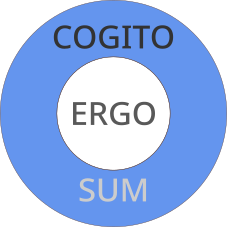
\includegraphics[width=0.6\textwidth,height=\textheight]{images/finalcut.svg}
\caption{Logo: the final cut}
\end{figure}

\hypertarget{finale}{%
\subsubsection{Finale}\label{finale}}

As he gazed upon his latest effort, Sol experienced the exultation and
closure felt at the end of a long and challenging quest. Yes, he had
indeed fulfilled his commission. The last two logos were chosen for
presentation to his distinguished philosophers: it was time to fix an
appointment with them. But one thing was certain: he was not going to
change any colours. He would let \emph{their} biases colour their logo!
And with that, he heaved a huge sigh of relief.

\hypertarget{illustrations}{%
\subsubsection{Illustrations}\label{illustrations}}

The statues of Socrates and Diotima shown in this blog are exhibited
outside the
\href{https://www.uwa.edu.au/theatres/venues/undercroft}{Undercroft} of
\href{https://www.uwa.edu.au/}{The University of Western Australia}.

Apart from highlighted code, all other illustrations were generated
using XeLaTeX and applicable
\href{https://ctan.org/pkg?lang=en}{packages}, including the
\href{https://github.com/pgf-tikz/pgf}{TikZ-PGF suite}. Much code that
is freely available on the Web was accessed for guidance on typesetting
these illustrations.

\hypertarget{feedback}{%
\subsection{Feedback}\label{feedback}}

Please \href{mailto:feedback.swanlotus@gmail.com}{email me} your
comments and corrections.

\noindent A PDF version of this article is
\href{./the-making-of-a-logo.pdf}{available for download here}:

\begin{normalsize}

\begin{ttfamily}

\url{https://swanlotus.netlify.app/blogs/the-making-of-a-logo.pdf}

\end{ttfamily}

\end{normalsize}

\hypertarget{bibliography}{%
\section*{References}\label{bibliography}}
\addcontentsline{toc}{section}{References}

\hypertarget{refs}{}
\begin{CSLReferences}{0}{0}
\leavevmode\vadjust pre{\hypertarget{ref-mann2019}{}}%
\CSLLeftMargin{{[}1{]} }
\CSLRightInline{A. Mann, {`{What Is String Theory?}'}, 20-Mar-2019.
{[}Online{]}. Available:
\url{https://www.livescience.com/65033-what-is-string-theory.html}.
{[}Accessed: 12-Nov-2020{]}}

\leavevmode\vadjust pre{\hypertarget{ref-wood2019}{}}%
\CSLLeftMargin{{[}2{]} }
\CSLRightInline{C. Wood, {`{What Is String Theory?}: Reference article:
A simplified explanation and brief history of string theory'},
11-Jul-2019. {[}Online{]}. Available:
\url{https://www.space.com/17594-string-theory.html}. {[}Accessed:
12-Nov-2020{]}}

\leavevmode\vadjust pre{\hypertarget{ref-jones2020}{}}%
\CSLLeftMargin{{[}3{]} }
\CSLRightInline{A. Z. Jones, {`{The Basics of String Theory}'},
02-Mar-2019. {[}Online{]}. Available:
\url{https://www.thoughtco.com/what-is-string-theory-2699363}.
{[}Accessed: 12-Nov-2020{]}}

\leavevmode\vadjust pre{\hypertarget{ref-siegel2015}{}}%
\CSLLeftMargin{{[}4{]} }
\CSLRightInline{E. Siegel, {`{Why String Theory Is Not A Scientific
Theory}'}, 23-Dec-2015. {[}Online{]}. Available:
\url{https://www.forbes.com/sites/startswithabang/2015/12/23/why-string-theory-is-not-science/}.
{[}Accessed: 12-Nov-2020{]}}

\leavevmode\vadjust pre{\hypertarget{ref-castelvecchi2016}{}}%
\CSLLeftMargin{{[}5{]} }
\CSLRightInline{D. Castelvecchi, {`{Feuding physicists turn to
philosophy for help}: String theory is at the heart of a debate over the
integrity of the scientific method itself'}, 05-Jan-2016. {[}Online{]}.
Available:
\url{https://www.nature.com/news/feuding-physicists-turn-to-philosophy-for-help-1.19076}.
{[}Accessed: 12-Nov-2020{]}}

\leavevmode\vadjust pre{\hypertarget{ref-alves2017}{}}%
\CSLLeftMargin{{[}6{]} }
\CSLRightInline{R. A. Batista and J. Primack, {`{Is String theory
falsifiable?}: Can a theory that isn't completely testable still be
useful to physics?'} {[}Online{]}. Available:
\url{https://metafact.io/factchecks/30-is-string-theory-falsifiable}.
{[}Accessed: 12-Nov-2020{]}}

\leavevmode\vadjust pre{\hypertarget{ref-francis2019}{}}%
\CSLLeftMargin{{[}7{]} }
\CSLRightInline{M. R. Francis, {`{Falsifiability and physics}: Can a
theory that isn't completely testable still be useful to physics?'},
23-Apr-2019. {[}Online{]}. Available:
\url{https://www.scientificamerican.com/article/is-string-theory-science/}.
{[}Accessed: 12-Nov-2020{]}}

\leavevmode\vadjust pre{\hypertarget{ref-kuhn2012}{}}%
\CSLLeftMargin{{[}8{]} }
\CSLRightInline{T. S. Kuhn, \emph{{The Structure of Scientific
Revolutions}}, 50th Anniversary Edition. University of Chicago Press,
2012. }

\leavevmode\vadjust pre{\hypertarget{ref-bardi2007}{}}%
\CSLLeftMargin{{[}9{]} }
\CSLRightInline{J. S. Bardi, \emph{{The Calculus Wars: Newton, Leibniz,
and the Greatest Mathematical Clash of All}}, Illustrated Edition. Basic
Books, 2007. }

\leavevmode\vadjust pre{\hypertarget{ref-watson2020}{}}%
\CSLLeftMargin{{[}10{]} }
\CSLRightInline{R. A. Watson, {`René descartes'}, 10-Apr-2020.
{[}Online{]}. Available:
\url{https://www.britannica.com/biography/Rene-Descartes}. {[}Accessed:
12-Nov-2020{]}}

\end{CSLReferences}



\end{document}
